\documentclass[10pt,a4paper]{article}
\usepackage[utf8]{inputenc}
\usepackage{url}
\usepackage[english]{babel}
\usepackage{amsmath}
\usepackage{amsfonts}
\usepackage{amssymb}
 \usepackage{float}
\usepackage{graphicx}
\usepackage[left=2cm,right=2cm,top=2cm,bottom=2cm]{geometry}
\author{Andres Chaves}
\title{Research Proposal}

\begin{document}
 \title{Research Proposal}
 \author{Andres Chaves (706801) \\
  \multicolumn{1}{p{.7\textwidth}}{\centering\emph{Melbourne School of Information\\The University of Melbourne}}}
 \maketitle

\begin{abstract}
    The purpose of this documents is to establish the context and bases of my research proposal which applies concepts of Machine Learning into Network Management Systems.
   \\\\
   Throughout this document we will read the relevance of the research, how will the concepts of Machine Learning will be applied to Event-processing Network Management Systems and finally what are the expected results.
\end{abstract}


\tableofcontents

  
 \section{Introduction}
 There is no doubt on the strong development and evolution of Information Technologies in modern world. Nowadays, we have access to computing devices in several forms such as supercomputers, laptops, tablets and smart phones; also this device development comes in conjunction with  advanced distributed information systems.
 \\\\
 But this evolution could not be accomplished without a key component: Computer Networks. Networks make data exchange and information services consumption possible and side by side with Information Technology, networking has evolved from simple small low bandwidth networks, to high speed wired and wireless ones connecting all the world.
 \\\\
 These huge networks require a set of practices, tools and knowledge in order to guarantee the availability and quality of service required by clients. A discipline called Network Management has arisen to address all these previous concerns and nowadays Network Management comprises all the practices and activities that a carrier must perform in order to fulfill its Service Level Agreements (SLAs) with its clients.
 \\\\
 From the information systems perspective, Network Management requires a set of systems called Network Management Systems (NMS), designed to administer either all or a part of the network. These administration is composed by a set of functions: Fault Management, Performance Management, Configuration Management and Security Management among others.
 \\\\
 Fault Management involves how to detect, classify and inform network operators about conditions that affect or may affect the network services, both from availability and performance perspective. Typically, network elements inform this to an  information system in an asynchronous way using SNMP protocol, specifically a SNMP TRAP event.
 \\\\
 One of the challenges in Network Management is how to monitor ever bigger networks where there are network devices in the range of thousands to millions. With a network of this size the rate of alarms received by a system can be around hundreds of events per second and with this alarm rate a key desired function of a NMS is to only show the relevant alarms to the network operators.
 \\\\
 One possible approach to analyse, classify and display only the relevant events to the operator is by the use of a machine learning system that helps the network operator process events and thus augment the network management capacity with the same engineering team size.
 \\\\
 This project intends to advance in this approach and measure the likelihood in the use of a machine learning system to fault management.

 \section{Objective}
The objective of this project is to analyse how machine learning technologies can be applied to Network Management Systems, specifically event/fault management systems in order to reduce the alarm rate and report only key events to the network operator and thus increase their network management capacity of a Network Operation Center.
\\\\
The Machine Learning technique will be used for reducing the volume of alarms by suppressing correlated or secondary alarms for a given Network Event. The objective is not to replace the judge and knowledge of the engineer but quickly 
help him in discovering what correlation rules may be applied to reduce the ratio alarm to operator.

  \section{Problem Definition}
A fault management system (FMS) is a stream processor of Alarms where alarms are received, processed and displayed:
\\\\
\begin{figure}[H]
 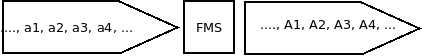
\includegraphics[scale=0.4]{NMS_FMS.png}
  \centering
  \caption{\textit{An abstraction of a Fault Management System}}
  \label{fig:nms_fms}
\end{figure}	

Whenever a relevant event happens on a Network, each Network Element sends alarms according to their role. A network event is translated into several alarms that may come from different sources. For example, if the event is a physical medium failure, the Transmission TX equipment will send an alarm reporting this, but also all the networks elements that rely on this equipments will perceive the event. In this sense for example, if a Switch equipment is related to the TX equipment then it will send a Layer 2 alarm and also a if Router is related then a Layer 3 alarm will be sent. We can see that a network event is translated into a cascade of different events and therefore given an event E1 the FMS system may receive several alarms from different network elements:
\\\\
\begin{figure}[H]
 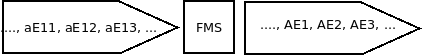
\includegraphics[scale=0.4]{NMS_FMS_EVENT.png}
  \centering
  \caption{\textit{A representation of the alarms of a given event arriving to a FMS}}
  \label{fig:nms_fms_event}
\end{figure}	

It is important to mention that several events can be happening at the same time in a network and thus the FMS receive a storm of alarms from different sources and also the alarms can be received in different order. The FMS is a system built to recognize alarms but is unable to identify which alarms belong to the same event:
\\\\
\begin{figure}[H]
 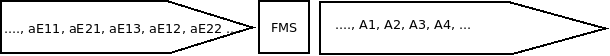
\includegraphics[scale=0.4]{NMS_FMS_EVENTS.png}
  \centering
  \caption{\textit{Several alarms from different events arriving to a FMS}}
  \label{fig:nms_fms_events}
\end{figure}	

Because the FMS is unable to recognize which alarms are related to the same event the volume of alarms presented to the network operator is dramatically high. In this sense, it is required a component in the FMS which allows the system to infer what alarms are related to the same event and then suppress them showing only one single alarm. However, it would be impractical to explicitly develop this component due to the number of different events present in a network, the number of possible alarms and the time required from the expert to analyze the relation between events and alarms.
\\\\
Given that the development of this component would be impractical a machine learning system is proposed to address the implementation of this component. A common definition of machine learning system is a computer system that can perform a function without being explicitly programmed \cite{netsnmp}. In this sense, we want a machine learning system as a component of the FMS which allows the system to infer what alarms are related to the same event and then suppress them showing only one single alarm. 
\\\\
More formally, we can represent our desired Machine Learning System as a function \textit{h} that receives the input stream of alarms and classifies whether the alarms are related to the same event:

\begin{figure}[H]
 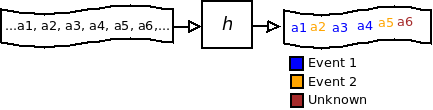
\includegraphics[scale=0.4]{MLS_hypothesis.png}
  \centering
  \caption{\textit{Representation of the proposed Machine Learning System}}
  \label{fig:mls_hypothesis}
\end{figure}	

Note that the system is not interested in to know what is the specific type of event but whether the alarms belong to the same event, whichever it is.

  \section{Proposed Solution}
  
- The network operator labels the alarm that he considers represent the event
AE13, AE12, AE22, AE23... -> FMS -> OPERATOR -> AE12

- The machine learning system prepares an input data set of unsupervised examples from the historical set of alarms with the labelled alarm present.
- The machine learning system runs an unsupervised learning algorithm in order to infer the correlation of the alarms in the set
- The machine learning systems present the results to the network operator
- The network operator determine if the correlation found is valid
- The correlation rules are added to the FMS, and whenever the labelled event arrives again the system will not present the correlated alarms.

  \section{Technical Approach}
A generic SNMP Fault Management System is a stream based system that conceptually can be divided into several stages: Alarm reception, alarm translation and enrichment, event correlation and event presentation. A conceptual schema can be seen on Figure \ref{fig:nms_generaldiagram}
\\\
\begin{figure}[H]
 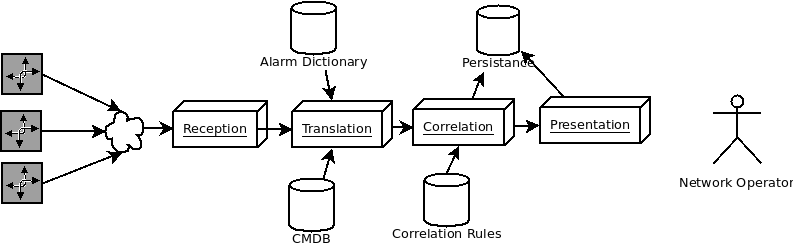
\includegraphics[scale=0.4]{NMS_GeneralDiagram.png}
  \centering
  \caption{\textit{A schematic of a generic Network Management System}}
  \label{fig:nms_generaldiagram}
\end{figure}	

For our testing environment we are going to use several open source components to simulate a Fault Management System. These are:

\begin{itemize}
  \item Net-SNMP: Net-SNMP is an open source Linux and Unix package that implements the SNMP protocol.\cite{netsnmp}
  \item SNMPTT: SNMPTT or SNMP-Trap Translator is an open source component that takes the SNMP trap (alarm) received by Net-SNMP and by using an alarm dictionary translate it into a more useful event. SNMPTT can also enrich the alarm from a database by executing a shell script.\cite{snmptt}
  \item MLS: Machine Learning System Component will be our learning algorithm.\cite{sec}
  \item MYSQL: MySQL is an open source relational database. For the purposes of this proposal, it will be used as storage for the Alarms and Configuration Management Database.
  \item Frontend: There will be a frontend to show the reduced alarms to network operators.
\end{itemize}

The recording will have a flag to indicate whether the operator consider the alarm is important or not. This field along with the context of the alarm (device, port, location, label) will be the input to the different machine learning algorithms. The output of the algorithms will be a set of inferred rules, that will be again evaluated and tested.
\\\\
The proposed components can be seen on figure \ref{fig:ml_componentdiagram}

\begin{figure}[H]
 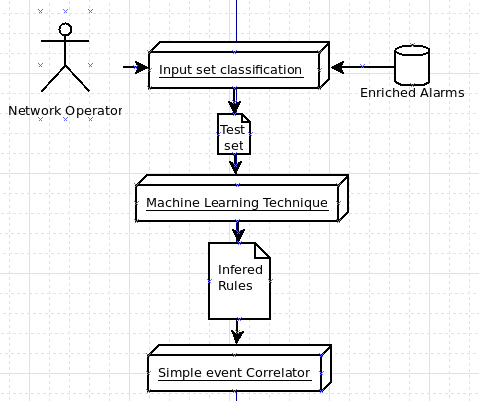
\includegraphics[scale=0.7]{ML_ProposedComponents.png}
  \centering
  \caption{\textit{Proposed Machine Learning Application}}
  \label{fig:ml_componentdiagram}
\end{figure}	

  \section{Time Table and Deliverables}
The research project is decomposed by the following tasks and deliverables:

\begin{center}
 \begin{tabular}{||c | c | c | c||} 
 \hline
 Task & Date & Deliverable \\ [0.7ex] 
 \hline\hline
 First version of Research Proposal  & 2014/11/24 & Yes \\ 
 \hline
 Initial Data Set Acquisition (without Classification) & 2014/12/05 & No \\ 
 \hline
 Establishing ML Techniques to be used & 2014/12/16 & No \\
 \hline
 Development of a quick prototype to classify alarms & 2014/12/26 & No \\
 \hline
 Data Set Acquisition (with Classification)  & 2015/01/09 & No \\
 \hline
 Final version of Research Proposal & 2015/02/24 & Yes \\ [1ex] 
 \hline
 Application of ML Techniques to the dataset & 2014/03/24 & No \\
 \hline
 Analysis of each ML technique & 2014/04/16 & No \\
 \hline
 First version of the final report (Thesis) & 2014/05/11 & Yes \\
 \hline
 Final version of the final report (Thesis) & 2014/05/29 & Yes \\

 \hline
\end{tabular}
\end{center}

  \section{Expected Results}

It is expected that the rules inferred Machine Learning Techniques be useful, accurate and general as possible in order to present only key events to Network Operators. Also it is expected a comparison between the different techniques tested.
\\\\
Normally, carriers buy expensive Network Management Systems, with correlation capabilities, but the lack of time or knowledge from Network Operators causes that to not take advantage of these powerful tools. With this approach, a set of rules can be generated and quickly incorporated into a Network Management System increasing its value added to the process of Network Management.

  \section{Literature Review}
As Network Management involves processing and analysis of large datasets there has been several attempts to use Machine Learning techniques to aid or improve this large analysis.
\\\\
The majority if the reviewed literature attempts to use Machine Learning into traffic flow analysis and Security. Traffic Analysis is one of the key parts in Network Management because it allows to determine patterns and behaviour segmented by type of traffic (HTTP, FTP, P2P, etc). For the security part the intention is to use Machine Learning to aid in the analysis of security logs to detect intrusion or attacks. While these topics are also part of Network Management the objectives and results differ with the purpose of this research.
\\\\
There are a couple of papers that have explored how to apply Machine Learning to alarm handling, The first one titled "Algorithm of Mining Fuzzy Association Rules in Network Management" attempts to reduce the volume of alarms in a event database by applying the theory of Fuzzy Sets to find the frequent sets and association rules between them.\cite{liu2003}.
\\\\
The second one, named "An Artificial Intelligence Approach to Network Fault Management" discuss what Artificial Intelligence methods can be applied to fault management and suggest the use of either Neural Networks or Bayesian Belief Networks to the problem \cite{kefferundef}.

\begin{thebibliography}{9}

\bibitem{mlwiki} Wikipedia definition of Machine Learning, \url{http://en.wikipedia.org/wiki/Machine_learning}.
\bibitem{netsnmp}Net-SNMP website, \url{http://www.net-snmp.org/}.
\bibitem{snmptt}SNMPTT website, \url{http://snmptt.sourceforge.net/docs/snmptt.shtml}.
\bibitem{sec}SEC website, \url{http://simple-evcorr.sourceforge.net}.
\bibitem{liu2003}
  Pei-Qi Liu, Zeng-Zhi Li, Yim-Liang Zhao,
  \emph{Algorithm of Mining Fuzzy Association Rules in Network Management}.
  Proceedings of the Second International Conference on Machine Learning and Cybernetics, Xi'an,
  2003.
\bibitem{kefferundef}
  Denise W. Gürer, Irfan Khan, Richard Ogier, Renee Keffer,
  \emph{An Artificial Intelligence Approach to Network Fault Management}.
  
\end{thebibliography}
    
\end{document}